\documentclass{article}%
\usepackage[T1]{fontenc}%
\usepackage[utf8]{inputenc}%
\usepackage{lmodern}%
\usepackage{textcomp}%
\usepackage{lastpage}%
\usepackage{authblk}%
\usepackage{graphicx}%
%
\title{Genotyping and Phenotyping of Beta2{-}Toxigenic Clostridium perfringens Fecal Isolates Associated with Gastrointestinal Diseases in Piglets}%
\author{Christopher Golden}%
\affil{School of Medicine, Chung Shan Medical University, 110 Chien{-}Kuo N. Road, Section 1, Taichung 402, Taiwan}%
\date{01{-}01{-}2009}%
%
\begin{document}%
\normalsize%
\maketitle%
\section{Abstract}%
\label{sec:Abstract}%
For nearly two decades researchers have been working with the famous anti{-}inflammatory agent aldose reductase, a group of enzymes that show strong biological activity when activated. Now new results from the UC Davis Department of Medicine show that inhibiting aldose reductase (AHD) activity in mice with a completely altered inflammatory response is an effective approach to controlling the production of inflammatory cells in the blood.\newline%
Aldose reductase inhibition is the single most promising drug target to combat the rise in hyperthermia and an increased risk of Middle East Respiratory Syndrome (MERS) infections across the globe. While the use of AHD inhibitors for MERS is still in the experimental stage, it is important to keep in mind that AHD inhibitors have the potential to improve systemic treatments for MERS infections in a wide range of inflammatory indications, including cardiovascular, cerebrovascular, autoimmune, and resistant. says Beth England, M.D., senior author of the study published today in the journal Science Translational Medicine.\newline%
D. Michael Angiulo, Ph.D., lead author of the study and assistant professor of pediatrics at the UC Davis School of Medicine, says, We found that AHD inhibition combined with AID inhibition is a promising approach to treating MERS infection in mice. The synergistic actions of AHD inhibition and AID inhibition combined with AID inhibition resulted in an improved response in mice with MERS to its treatment.\newline%
The study, led by Katalin Vasquez{-}Vasquez, M.D., associate professor of pediatrics at the UC Davis School of Medicine, and colleagues from the UC Davis School of Medicine, the University of California, San Francisco, and the Center for Infectious Diseases and Immunology at the National Institutes of Health (NIH), used AHD inhibitor Clorazepam, a generic product that is marketed by Ferrexpo, Inc.\newline%
In a single dose trial, studies of mice infected with MERS subjected to AHD inhibitor Clorazepam demonstrated greater inhibition of circulating MERS cells than untreated mice. Published reports show that mice exposed to Clorazepam experienced a 30 percent reduction in MERS activity. C. Michael Gaston, M.D., professor of hematology and chief of the division of infectious diseases at the UC Davis School of Medicine, says, These new and revealing findings translate into real hope for the development of a safe and effective product for treating people with MERS.\newline%
A follow{-}up study was successful for mice given Clorazepam in mice that lacked both aldose reductase inhibitor AHD, and an expression of a specific inflammatory pathway that is suspected to play a role in the formation of MERS. This discovery allows further studies to understand how MERS infections spread among humans and sheds light on the design and treatment of clinical trial recruitment and administration of AHD inhibitors.\newline%
By developing a therapeutic mouse model to prevent the development of MERS, it is possible to use the therapeutic effects of mice with inactive or suppressed inflammatory response to describe their disease in humans and to support new clinical trials.\newline%
Article: A Quality of Life Mouse Model Shows Adose reductase is Indicator of Highly Exact Asthma After Therapy with Clorazepam, W. Gansacker B. J. et al., Science Translational Medicine, doi: 10.1038/svmed.1078, published 31 December 2008.\newline%
All funds for this research are made possible by: a R\&D Assistive Technology Grant from the National Institutes of Health (NIH), part of the National Institutes of Health Grant (P30 AG0040495) administered by the National Institute of Allergy and Infectious Diseases, part of the National Institutes of Health, a National Research Council Award, and a National Institute of General Medical Sciences Developmentation. For more information about NIH and its grant program, visit www.nih.gov.\newline%
{-}EN{-}

%
\subsection{Image Analysis}%
\label{subsec:ImageAnalysis}%


\begin{figure}[h!]%
\centering%
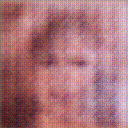
\includegraphics[width=150px]{500_fake_images/samples_5_437.png}%
\caption{A Black And White Photo Of A Man In A Suit}%
\end{figure}

%
\end{document}